% questions.tex —— 2000 年·春季京皖卷·文科 · 题目内容片段（无答案）
% 由 tools/generate_projects.py 依来源总账自 2000/2000_数学真题_春季京皖文_试题.md 生成，勿手改（改源 MD 后重跑）


\gkpart{数学}

\begin{gktip}
\textbf{来源说明}：依据固定源 PDF 的原生文字层逐题转录，并对照 300 dpi 渲染与内容流核对（补集上划线、向量箭头、根号横、分数线为矢量短线，不在文字层）。源为 \textbf{XeTeX 重排件（非扫描）}，2 页 A3 横向三栏，页脚印刷页码 63、64；无答案页。题号 1–24 连续：选择 1–14、填空 15–18、解答 19–24。

\textbf{源内疑点}（照录不补正）：第 18 题 ③ 原页作「都有垂直」（「都」与「有」之间无停顿），疑为「都垂直」之误，照录不补正；第 24 题「年用电量为 a kW·h 本年度计划…」与「0.4 元/kW·h 经测算…」两处缺标点，原页如此，照录未补。

\textbf{图示}：第 14 题三次函数图象、第 21 题折叠三视图（3 幅）、第 23 题抛物线均由源内容流逐路径重绘，线宽/虚线按源值。
\end{gktip}

\gkpart{一、选择题}

\begin{question}
\gkti{1}复数 $z_1 = 3 + \mathrm{i}$，$z_2 = 1 - \mathrm{i}$，则 $z = z_1 \cdot z_2$ 在复平面内的对应点位于　（　）

\begin{gkopts}(4)
\task （A）第一象限
\task （B）第二象限
\task （C）第三象限
\task （D）第四象限
\end{gkopts}

\end{question}
\begin{question}
\gkti{2}设全集 $I = \{a, b, c, d, e\}$，集合 $M = \{a, c, d\}$，$N = \{b, d, e\}$，那么 $\overline{M} \cap \overline{N}$ 是　（　）

\begin{gkopts}(4)
\task （A）$\varnothing$
\task （B）$\{d\}$
\task （C）$\{a, c\}$
\task （D）$\{b, e\}$
\end{gkopts}

\end{question}
\begin{question}
\gkti{3}已知双曲线 $\frac{x^2}{b^2} - \frac{y^2}{a^2} = 1$ 的两条渐近线互相垂直，那么该双曲线的离心率是　（　）

\begin{gkopts}(4)
\task （A）$2$
\task （B）$\sqrt{3}$
\task （C）$\sqrt{2}$
\task （D）$\frac{3}{2}$
\end{gkopts}

\end{question}
\begin{question}
\gkti{4}下列方程关于 $x = y$ 对称的是　（　）

（A）$x^2 - x + y^2 = 1$　（B）$x^2 y + x y^2 = 1$

（C）$x - y = 1$　（D）$x^2 - y^2 = 1$

\end{question}
\begin{question}
\gkti{5}一个圆锥的底面直径和高都同一个球的直径相等，那么圆锥与球的体积之比是　（　）

\begin{gkopts}(4)
\task （A）$1:3$
\task （B）$2:3$
\task （C）$1:2$
\task （D）$2:9$
\end{gkopts}

\end{question}
\begin{question}
\gkti{6}直线 $(\sqrt{3} - \sqrt{2})x + y = 3$ 和直线 $x + (\sqrt{2} - \sqrt{3})y = 2$ 的位置关系是　（　）

\begin{gkopts}(2)
\task （A）相交但不垂直
\task （B）垂直
\task （C）平行
\task （D）重合
\end{gkopts}

\end{question}
\begin{question}
\gkti{7}函数 $y = \lg |x|$　（　）

（A）是偶函数，在区间 $(-\infty, 0)$ 上单调递增

（B）是偶函数，在区间 $(-\infty, 0)$ 上单调递减

（C）是奇函数，在区间 $(0, +\infty)$ 上单调递增

（D）是奇函数，在区间 $(0, +\infty)$ 上单调递减

\end{question}
\begin{question}
\gkti{8}从单词“equation”选取 5 个不同的字母排成一排，含有“qu”（其中“qu”相连且顺序不变）的不同排列共有　（　）

\begin{gkopts}(4)
\task （A）120 个
\task （B）480 个
\task （C）720 个
\task （D）840 个
\end{gkopts}

\end{question}
\begin{question}
\gkti{9}椭圆短轴长是 2，长轴长是短轴的 2 倍，则椭圆中心到其准线距离是　（　）

\begin{gkopts}(2)
\task （A）$\frac{8}{5}\sqrt{5}$
\task （B）$\frac{4}{5}\sqrt{5}$
\task （C）$\frac{8}{3}\sqrt{3}$
\task （D）$\frac{4}{3}\sqrt{3}$
\end{gkopts}

\end{question}
\begin{question}
\gkti{10}函数 $y = \sin x + \cos x + 2$ 的最小值是　（　）

\begin{gkopts}(4)
\task （A）$2 - \sqrt{2}$
\task （B）$2 + \sqrt{2}$
\task （C）$0$
\task （D）$1$
\end{gkopts}

\end{question}
\begin{question}
\gkti{11}设复数 $z_1 = -1 - \mathrm{i}$ 在复平面上对应向量 $\overrightarrow{OZ_1}$，将 $\overrightarrow{OZ_1}$ 按顺时针方向旋转 $\frac{5}{6}\pi$ 后得到向量 $\overrightarrow{OZ_2}$，令 $\overrightarrow{OZ_2}$ 对应的复数为 $z_2$ 的辐角主值为 $\theta$，则 $\tan\theta =$　（　）

\begin{gkopts}(2)
\task （A）$2 - \sqrt{3}$
\task （B）$-2 + \sqrt{3}$
\task （C）$2 + \sqrt{3}$
\task （D）$-2 - \sqrt{3}$
\end{gkopts}

\end{question}
\begin{question}
\gkti{12}设 $\alpha$，$\beta$ 是一个钝角三角形的两个锐角，下列四个不等式中不正确的是　（　）

（A）$\tan\alpha \tan\beta < 1$　（B）$\sin\alpha + \sin\beta < \sqrt{2}$

（C）$\cos\alpha + \cos\beta > 1$　（D）$\frac{1}{2}\tan(\alpha+\beta) < \tan\frac{\alpha+\beta}{2}$

\end{question}
\begin{question}
\gkti{13}已知等差数列 $\{a_n\}$ 满足 $a_1 + a_2 + a_3 + \cdots + a_{101} = 0$，则有　（　）

\begin{gkopts}(2)
\task （A）$a_1 + a_{101} > 0$
\task （B）$a_2 + a_{100} < 0$
\task （C）$a_3 + a_{99} = 0$
\task （D）$a_{51} = 51$
\end{gkopts}

\Needspace{0.4\textheight}
\end{question}
\begin{question}
\gkti{14}已知函数 $f(x) = ax^3 + bx^2 + cx + d$ 的图象如图，则　（　）
\nopagebreak[4]
\begin{center}% ============================================================================
% 2000 年春季高考（京、皖）文科 第 14 题：三次函数 y = f(x) 的图象
% ----------------------------------------------------------------------------
% 来源：.work/phase4-b20/source/2000春季京皖文.pdf
%       SHA-256 b9552b8354735296f6ea1ed051085e094e4af0c14ff97ada2dbd4e579b14287f
%       第 1 页，内容流对象 39 / 40 / 42 / 43 / 44 / 45 / 46 / 47（按页面资源顺序拼接解析）
% 重绘方式：qpdf --qdf 取内容流 → 解析 m/l/c/re/S/f、w、d → 本地坐标
%          本地坐标 = 页面坐标 − (608.528, 616.430)，原点取坐标轴交点 O；
%          1 单位 = 1 TeX pt；页面为 A3（1190.55 × 841.89 pt）。
% 元素计数：实线路径 3（x 轴、y 轴、函数曲线），填充箭头 2，虚线路径 0，标签 5（y, O, 1, 2, x）
% 线宽：轴 0.40 pt；曲线 0.80 pt（内容流 w=0.79701）；箭头填充三角形长 3.99 pt、半宽 1.49 pt
% 坐标基准与源位的偏差：端点四舍五入到 0.001 pt；曲线按 299 段三次 Bézier 采样的折线重绘，经 0.02 pt 容差简化（57 点），最大偏差 < 0.02 pt。
% 标签：位置 = pdftotext -bbox 文本中心 − 基准；O 源位 (−7.998,−8.250)，左移 3.0 pt；1、2 源位 (17.012,−7.840)/(34.012,−7.840)，同步下移 2.4 pt；x 源位 (51.022,−5.590)，下移 1.8 pt；y 未动。净距均 ≥ 2 pt
% ============================================================================
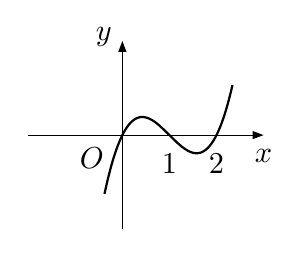
\begin{tikzpicture}[x=1pt, y=1pt,
    every node/.style={inner sep=0pt, font=\fontsize{10.5pt}{12.6pt}\selectfont}]
  % --- 坐标轴（轴身止于箭头底边，箭头为内容流中的独立填充三角形）
  \draw[line width=0.4pt] (-34.017,0) -- (47.438,0); % x 轴轴身
  \fill (51.025,0) -- (47.040,1.494) -- (47.040,-1.494) -- cycle; % x 箭头
  \draw[line width=0.4pt] (0,-34.017) -- (0,30.430); % y 轴轴身
  \fill (0,34.016) -- (1.494,30.031) -- (-1.494,30.031) -- cycle; % y 箭头
  % --- 三次函数曲线（内容流 299 段三次 Bézier → 0.02pt 容差 57 点折线）
  \draw[line width=0.8pt]
      (-6.463,-21.227) -- (-5.299,-16.066) -- (-4.112,-11.446) -- (-3.514,-9.357) -- (-2.894,-7.348) -- (-2.273,-5.498) --
      (-1.641,-3.772) -- (-1.020,-2.227) -- (-0.387,-0.801) -- (0.274,0.534) -- (0.936,1.721) -- (1.596,2.756) --
      (2.264,3.664) -- (2.954,4.458) -- (3.648,5.117) -- (4.364,5.656) -- (5.085,6.064) -- (5.809,6.343) --
      (6.573,6.507) -- (7.349,6.544) -- (8.125,6.460) -- (8.938,6.253) -- (9.783,5.921) -- (10.572,5.514) --
      (11.396,5.001) -- (12.266,4.374) -- (13.197,3.620) -- (15.059,1.923) -- (18.487,-1.468) -- (19.931,-2.837) --
      (21.408,-4.106) -- (22.104,-4.638) -- (22.791,-5.114) -- (23.581,-5.591) -- (24.343,-5.971) -- (25.065,-6.249) --
      (25.781,-6.439) -- (26.488,-6.535) -- (27.151,-6.536) -- (27.812,-6.445) -- (28.456,-6.262) -- (29.243,-5.904) --
      (30.019,-5.397) -- (30.784,-4.739) -- (31.549,-3.914) -- (32.286,-2.951) -- (33.006,-1.844) -- (33.721,-0.575) --
      (34.431,0.859) -- (35.118,2.422) -- (35.800,4.147) -- (36.490,6.077) -- (37.158,8.131) -- (37.817,10.340) --
      (38.494,12.801) -- (39.153,15.395) -- (39.785,18.071);
  % --- 标签
  \node at (-6.648,35.400) {$y$};
  \node at (-10.998,-8.250) {$O$};
  \node at (17.012,-10.240) {$1$};
  \node at (34.012,-10.240) {$2$};
  \node at (51.022,-7.390) {$x$};
\end{tikzpicture}
% ----------------------------------------------------------------------------
% 自验：轴端点 (−34.017,0)/(47.438,0) 与 (0,−34.017)/(0,30.430) 和内容流 574.5115/655.9662/582.4135/646.86 逐点吻合；曲线 57 点对源 Bézier 的最大偏差 < 0.02 pt；曲线与 x 轴交点 local x = −0.015 / 17.038 / 34.002，与标签 1、2 的横坐标 17.012 / 34.012 一致（偏差 < 0.03 pt）。标签净距（字形墨迹包围盒对路径中心线，已扣除线宽半宽）：y 3.30、O 2.14、1 4.00、2 2.41、x 2.95 pt，均 ≥ 2 pt。探针编译：xelatex 0 错误、0 警告。
% ============================================================================
\end{center}
\nopagebreak[4]
\begin{gkopts}(2)
\task （A）$b \in (-\infty, 0)$
\task （B）$b \in (0, 1)$
\task （C）$b \in (1, 2)$
\task （D）$b \in (2, +\infty)$
\end{gkopts}

\end{question}
\gkpart{二、填空题}

\begin{question}
\gkti{15}函数 $y = \cos\left(\frac{2\pi}{3}x + \frac{\pi}{4}\right)$ 的最小正周期是\gkblank{}．

\end{question}
\begin{question}
\gkti{16}已知一体积为 72 的正四面体，连结两个面的重心 $E$、$F$，则线段 $EF$ 的长是\gkblank{}．

\end{question}
\begin{question}
\gkti{17}$\left(\sqrt{x} - \frac{1}{\sqrt[3]{x}}\right)^{10}$ 展开式中的常数项是\gkblank{}．

\end{question}
\begin{question}
\gkti{18}在空间，下列命题正确的是\gkblank{}．（注：把你认为正确的命题的序号都填上）

① 如果两直线 $a$、$b$ 分别与直线 $l$ 平行，那么 $a \parallel b$；

② 如果直线 $a$ 与平面 $\beta$ 内的一条直线 $b$ 平行，那么 $a \parallel \beta$；

③ 如果直线 $a$ 与平面 $\beta$ 内的两条直线 $b$、$c$ 都有垂直，那么 $a \perp \beta$；

④ 如果平面 $\beta$ 内的一条直线 $a$ 垂直平面 $\gamma$，那么 $\beta \perp \gamma$．

\end{question}
\gkpart{三、解答题}

\begin{question}
\gkti{19}已知二次函数 $f(x) = (\lg a)x^2 + 2x + 4\lg a$ 的最大值为 3，求 $a$ 的值．

\end{question}
\begin{question}
\gkti{20}在 $\triangle ABC$ 中，角 $A$、$B$、$C$ 对边分别为 $a$、$b$、$c$，证明：$\dfrac{a^2 - b^2}{c^2} = \dfrac{\sin(A - B)}{\sin C}$．

\Needspace{0.4\textheight}
\end{question}
\begin{question}
\gkti{21}在直角梯形 $ABCD$ 中，$\angle D = \angle BAD = 90^\circ$，$AD = DC = \frac{1}{2}AB = a$（如图一）．将 $\triangle ADC$ 沿 $AC$ 折起，使 $D$ 到 $D'$．记面 $ACD'$ 为 $\alpha$，面 $ABC$ 为 $\beta$，面 $BCD'$ 为 $\gamma$．

（1） 若二面角 $\alpha-AC-\beta$ 为直二面角（如图二），求二面角 $\beta-BC-\gamma$ 的大小；

（2） 若二面角 $\alpha-AC-\beta$ 为 $60^\circ$（如图三），求三棱锥 $D'-ABC$ 的体积．
\nopagebreak[4]
\begin{center}% ============================================================================
% 2000 年春季高考（京、皖）文科 第 21 题 图一：直角梯形 ABCD
% ----------------------------------------------------------------------------
% 来源：.work/phase4-b20/source/2000春季京皖文.pdf
%       SHA-256 b9552b8354735296f6ea1ed051085e094e4af0c14ff97ada2dbd4e579b14287f
%       第 1 页，内容流对象 47（图注「图一」为排版文字，不在本图内）
% 重绘方式：qpdf --qdf 取内容流 → 解析 m/l/c/re/S/f、w、d → 本地坐标
%          本地坐标 = 页面坐标 − (874.160, 359.960)，原点取顶点 A（梯形左下角）；
%          1 单位 = 1 TeX pt；页面为 A3（1190.55 × 841.89 pt）。
% 元素计数：实线路径 4（AB、BC、CD、DA），虚线路径 1（AC），标签 4（A, B, C, D）
% 线宽：全部 0.40 pt；虚线 on/off 各 2.99 pt
% 坐标基准与源位的偏差：端点四舍五入到 0.001 pt；全部为直线段，无简化。
% 标签：位置 = pdftotext -bbox 文本中心 − 基准；D 源位 (−5.070,37.990)，左移 1.6 pt；C 源位 (38.580,37.990)，右移 1.0 pt、上移 2.2 pt；A、B 未动。净距均 ≥ 2 pt
% ============================================================================
\begin{tikzpicture}[x=1pt, y=1pt,
    every node/.style={inner sep=0pt, font=\fontsize{10.5pt}{12.6pt}\selectfont}]
  % --- 实线：AB、BC、CD、DA（内容流顺序为 AB→BC→CD→DA）
  \draw[line width=0.4pt] (0,0) -- (68.040,0);
  \draw[line width=0.4pt] (68.040,0) -- (34.020,34.020);
  \draw[line width=0.4pt] (34.020,34.020) -- (0,34.020);
  \draw[line width=0.4pt] (0,34.020) -- (0,0);
  % --- 虚线：AC（划长 2.99 pt，内容流 [2.98883 2.98883] 0 d）
  \draw[line width=0.4pt, dash pattern=on 2.99pt off 2.99pt] (0,0) -- (34.020,34.020);
  % --- 标签
  \node at (-6.670,37.990) {$D$};
  \node at (39.580,40.190) {$C$};
  \node at (-4.930,-5.890) {$A$};
  \node at (72.710,-5.890) {$B$};
  % 图注（源页图下居中；主会话添加）
  \node at (34.020,-12.000) {图一};
\end{tikzpicture}
% ----------------------------------------------------------------------------
% 自验：A=(0,0)、B=(68.040,0)、C=(34.020,34.020)、D=(0,34.020)，与内容流 874.16/942.20/908.18/874.16、359.96/393.98 逐点吻合；AD=DC=34.020、AB=68.040，满足题设 AD=DC=½AB；标签：A、B 取源位；D 左移 1.6 pt、C 右移 1.0 pt 并上移 2.2 pt。净距 A 3.32、B 3.22、D 2.44、C 2.18 pt。探针编译：0 错误、0 警告。
% ============================================================================
\end{center}
\nopagebreak[4]
\nopagebreak[4]
\begin{center}% ============================================================================
% 2000 年春季高考（京、皖）文科 第 21 题 图二：折叠后三棱锥 D′-ABC（直二面角）
% ----------------------------------------------------------------------------
% 来源：.work/phase4-b20/source/2000春季京皖文.pdf
%       SHA-256 b9552b8354735296f6ea1ed051085e094e4af0c14ff97ada2dbd4e579b14287f
%       第 1 页，内容流对象 47（图注「图二」不在本图内）
% 重绘方式：qpdf --qdf 取内容流 → 解析 m/l/c/re/S/f、w、d → 本地坐标
%          本地坐标 = 页面坐标 − (970.740, 359.960)，原点取顶点 A；
%          1 单位 = 1 TeX pt；页面为 A3（1190.55 × 841.89 pt）。
% 元素计数：实线路径 3（AB、BD′、D′A），虚线路径 3（AC、BC、CD′），标签 4（A, B, C, D′）
% 线宽：全部 0.40 pt；虚线 on/off 各 2.99 pt
% 坐标基准与源位的偏差：端点四舍五入到 0.001 pt；全部为直线段，无简化。
% 标签：位置 = pdftotext -bbox 文本中心 − 基准；C、D′ 取「字母 + 撇」合成包围盒中心（撇号在内容流中为独立 F9 字形，pdftotext 未单列）；C 源位 (21.920,14.130)，右移 2.4 pt、下移 3.4 pt；其余未动。净距均 ≥ 2 pt
% ============================================================================
\begin{tikzpicture}[x=1pt, y=1pt,
    every node/.style={inner sep=0pt, font=\fontsize{10.5pt}{12.6pt}\selectfont}]
  % --- 实线：AB、BD′、D′A
  \draw[line width=0.4pt] (0,0) -- (68.040,0);
  \draw[line width=0.4pt] (68.040,0) -- (17.010,34.020);
  \draw[line width=0.4pt] (17.010,34.020) -- (0,0);
  % --- 虚线：AC、BC、CD′
  \draw[line width=0.4pt, dash pattern=on 2.99pt off 2.99pt] (0,0) -- (20.410,20.410);
  \draw[line width=0.4pt, dash pattern=on 2.99pt off 2.99pt] (68.040,0) -- (20.410,20.410);
  \draw[line width=0.4pt, dash pattern=on 2.99pt off 2.99pt] (20.410,20.410) -- (17.010,34.020);
  % --- 标签
  \node at (-4.930,-5.890) {$A$};
  \node at (72.710,-5.890) {$B$};
  \node at (16.760,41.350) {$D'$};
  \node at (24.320,10.730) {$C$};
  % 图注（源页图下居中；主会话添加）
  \node at (34.020,-12.000) {图二};
\end{tikzpicture}
% ----------------------------------------------------------------------------
% 自验：A=(0,0)、B=(68.040,0)、D′=(17.010,34.020)、C=(20.410,20.410)，与内容流 970.74/1038.78/987.75/991.15、359.96/393.98/380.37 逐点吻合；D′ 到 A、B 的距离分别 38.03、61.33 pt，C 由三条虚线汇于一点；标签：A、B、D′ 取源位；C 合成中心 (992.66,374.09) 右移 2.4 pt、下移 3.4 pt。净距 A 3.31、B 3.23、D′ 3.71、C 2.26 pt。探针编译：0 错误、0 警告。
% ============================================================================
\end{center}
\nopagebreak[4]
\nopagebreak[4]
\begin{center}% ============================================================================
% 2000 年春季高考（京、皖）文科 第 21 题 图三：折叠后三棱锥 D′-ABC（二面角 60°）
% ----------------------------------------------------------------------------
% 来源：.work/phase4-b20/source/2000春季京皖文.pdf
%       SHA-256 b9552b8354735296f6ea1ed051085e094e4af0c14ff97ada2dbd4e579b14287f
%       第 1 页，内容流对象 47（图注「图三」不在本图内）
% 重绘方式：qpdf --qdf 取内容流 → 解析 m/l/c/re/S/f、w、d → 本地坐标
%          本地坐标 = 页面坐标 − (1067.320, 359.960)，原点取顶点 A；
%          1 单位 = 1 TeX pt；页面为 A3（1190.55 × 841.89 pt）。
% 元素计数：实线路径 3（AB、BD′、D′A），虚线路径 3（AC、BC、CD′），标签 4（A, B, C, D′）
% 线宽：全部 0.40 pt；虚线 on/off 各 2.99 pt
% 坐标基准与源位的偏差：端点四舍五入到 0.001 pt；全部为直线段，无简化。
% 标签：位置 = pdftotext -bbox 文本中心 − 基准；C、D′ 取「字母 + 撇」合成包围盒中心（撇号在内容流中为独立 F9 字形，pdftotext 未单列）；C 源位 (21.930,14.125)，右移 2.4 pt、下移 3.4 pt；其余未动。净距均 ≥ 2 pt
% ============================================================================
\begin{tikzpicture}[x=1pt, y=1pt,
    every node/.style={inner sep=0pt, font=\fontsize{10.5pt}{12.6pt}\selectfont}]
  % --- 实线：AB、BD′、D′A
  \draw[line width=0.4pt] (0,0) -- (68.040,0);
  \draw[line width=0.4pt] (68.040,0) -- (25.510,34.020);
  \draw[line width=0.4pt] (25.510,34.020) -- (0,0);
  % --- 虚线：AC、BC、CD′
  \draw[line width=0.4pt, dash pattern=on 2.99pt off 2.99pt] (0,0) -- (20.410,20.410);
  \draw[line width=0.4pt, dash pattern=on 2.99pt off 2.99pt] (68.040,0) -- (20.410,20.410);
  \draw[line width=0.4pt, dash pattern=on 2.99pt off 2.99pt] (20.410,20.410) -- (25.510,34.020);
  % --- 标签
  \node at (-4.930,-5.890) {$A$};
  \node at (72.700,-5.890) {$B$};
  \node at (25.265,41.350) {$D'$};
  \node at (24.330,10.725) {$C$};
  % 图注（源页图下居中；主会话添加）
  \node at (34.020,-12.000) {图三};
\end{tikzpicture}
% ----------------------------------------------------------------------------
% 自验：A=(0,0)、B=(68.040,0)、D′=(25.510,34.020)、C=(20.410,20.410)，与内容流 1067.32/1135.36/1092.83/1087.73、359.96/393.98/380.37 逐点吻合；D′ 的横坐标较图二右移 8.50 pt（60° 情形），C 位置与图二相同；标签合成中心 D′=(1092.585,401.31)、C=(1089.25,374.09)，换算后为 (25.265,41.350)、(21.930,14.125)；C 另右移 2.4 pt、下移 3.4 pt。净距 A 3.30、B 3.23、D′ 3.71、C 2.25 pt。探针编译：0 错误、0 警告。
% ============================================================================
\end{center}
\nopagebreak[4]
\end{question}
\begin{question}
\gkti{22}已知等差数列 $\{a_n\}$ 的公差和等比数列 $\{b_n\}$ 的公比相等，且都等于 $d$（$d > 0$，$d \neq 1$），若 $a_1 = b_1$，$a_3 = 3b_3$，$a_5 = 5b_5$，求 $a_n$，$b_n$．

\Needspace{0.4\textheight}
\end{question}
\begin{question}
\gkti{23}如图，设点 $A$ 和 $B$ 为抛物线 $y^2 = 4px$（$p > 0$）上原点以外的两个动点，已知 $OA \perp OB$，$OM \perp AB$．求点 $M$ 的轨迹方程，并说明它表示什么曲线．
\nopagebreak[4]
\begin{center}% ============================================================================
% 2000 年春季高考（京、皖）文科 第 23 题：抛物线 y² = 4px 与点 A、B、M
% ----------------------------------------------------------------------------
% 来源：.work/phase4-b20/source/2000春季京皖文.pdf
%       SHA-256 b9552b8354735296f6ea1ed051085e094e4af0c14ff97ada2dbd4e579b14287f
%       第 2 页，内容流对象 2
% 重绘方式：qpdf --qdf 取内容流 → 解析 m/l/c/re/S/f、w、d → 本地坐标
%          本地坐标 = 页面坐标 − (701.132, 687.581)，原点取坐标原点 O；
%          1 单位 = 1 TeX pt；页面为 A3（1190.55 × 841.89 pt）。
% 元素计数：实线路径 8（x 轴、y 轴、抛物线上支、下支、OA、OB、AB、OM），填充箭头 2，虚线 0，标签 6（O, A, B, M, x, y）
% 线宽：轴与辅助线 0.40 pt；抛物线两支 0.80 pt（内容流 w=0.79701）；箭头填充三角形长 3.99 pt、半宽 1.49 pt
% 坐标基准与源位的偏差：端点四舍五入到 0.001 pt；抛物线两支按 24 段三次 Bézier 采样的折线重绘，经 0.02 pt 容差简化（每支 32 点），最大偏差 < 0.02 pt。
% 标签：位置 = pdftotext -bbox 文本中心 − 基准；O、A、B、M、y 未动；x 源位 (68.578,−5.591)，下移 1.6 pt。净距均 ≥ 2 pt
% ============================================================================
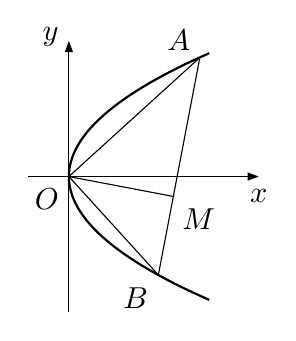
\begin{tikzpicture}[x=1pt, y=1pt,
    every node/.style={inner sep=0pt, font=\fontsize{10.5pt}{12.6pt}\selectfont}]
  % --- 坐标轴（轴身止于箭头底边，箭头为独立填充三角形）
  \draw[line width=0.4pt] (-14.695,0) -- (64.989,0); % x 轴轴身
  \fill (68.576,0) -- (64.591,1.494) -- (64.591,-1.494) -- cycle; % x 箭头
  \draw[line width=0.4pt] (0,-48.983) -- (0,45.396); % y 轴轴身
  \fill (0,48.983) -- (1.494,44.998) -- (-1.494,44.998) -- cycle; % y 箭头
  % --- 抛物线 y^2=4px 上、下两支（内容流 24 段三次 Bézier → 0.02pt 容差 32 点折线）
  \draw[line width=0.8pt]
      (0.000,0.000) -- (0.076,1.712) -- (0.202,2.786) -- (0.408,3.995) -- (0.792,5.572) -- (1.305,7.148) --
      (1.786,8.357) -- (2.337,9.567) -- (3.169,11.143) -- (4.130,12.720) -- (4.955,13.929) -- (5.849,15.138) --
      (7.129,16.715) -- (8.539,18.291) -- (9.708,19.500) -- (10.946,20.710) -- (12.675,22.286) -- (14.532,23.863) --
      (16.045,25.072) -- (17.627,26.281) -- (19.804,27.858) -- (22.110,29.434) -- (23.967,30.644) -- (25.893,31.853) --
      (28.518,33.429) -- (31.272,35.006) -- (33.473,36.215) -- (35.743,37.424) -- (38.816,39.001) -- (42.019,40.577) --
      (44.563,41.787) -- (50.699,44.572);
  \draw[line width=0.8pt]
      (0.000,0.000) -- (0.076,-1.712) -- (0.202,-2.786) -- (0.408,-3.995) -- (0.792,-5.572) -- (1.305,-7.148) --
      (1.786,-8.357) -- (2.337,-9.567) -- (3.169,-11.143) -- (4.130,-12.720) -- (4.955,-13.929) -- (5.849,-15.138) --
      (7.129,-16.715) -- (8.539,-18.291) -- (9.708,-19.500) -- (10.946,-20.710) -- (12.675,-22.286) -- (14.532,-23.863) --
      (16.045,-25.072) -- (17.627,-26.281) -- (19.804,-27.858) -- (22.110,-29.434) -- (23.967,-30.644) -- (25.893,-31.853) --
      (28.518,-33.429) -- (31.272,-35.006) -- (33.473,-36.215) -- (35.743,-37.424) -- (38.816,-39.001) -- (42.019,-40.577) --
      (44.563,-41.787) -- (50.699,-44.572);
  % --- 辅助线：OA、OB、AB、OM
  \draw[line width=0.4pt] (0,0) -- (47.317,43.007);   % OA
  \draw[line width=0.4pt] (0,0) -- (32.329,-35.562);  % OB
  \draw[line width=0.4pt] (32.329,-35.562) -- (47.317,43.007); % AB
  \draw[line width=0.4pt] (0,0) -- (38.108,-7.270);   % OM ⊥ AB
  % --- 标签
  \node at (-7.990,-8.250) {$O$};
  \node at (39.680,49.330) {$A$};
  \node at (24.120,-43.810) {$B$};
  \node at (46.900,-15.520) {$M$};
  \node at (68.580,-7.190) {$x$};
  \node at (-6.650,50.370) {$y$};
\end{tikzpicture}
% ----------------------------------------------------------------------------
% 自验：A=(47.317,43.007) 即页面 (748.449,730.588)、B=(32.329,−35.562) 即 (733.460,652.020)、M=(38.108,−7.270) 即 (739.240,680.311)，均在内容流端点 0.001 pt 内；OA·OB = 0.0（OA⊥OB），OM·AB = 0.0（OM⊥AB，|OM| = 38.795 pt）；两支对 x = 0.025521·y² 的最大残差 0.012 pt（y² = 4px，p ≈ 9.80 pt），两支端点 (50.699,±44.572) 与源 (751.831,732.153)/(751.831,643.009) 吻合。标签：O、A、B、M、y 取源位，x 下移 1.6 pt；净距 O 3.89、A 2.41、B 6.58、M 5.11、x 2.98、y 3.44 pt。探针编译：0 错误、0 警告。
% ============================================================================
\end{center}
\nopagebreak[4]
\end{question}
\begin{question}
\gkti{24}某地区上年度电价为 $0.8$ 元/kW$\cdot$h，年用电量为 $a$ kW$\cdot$h　本年度计划将电价降到 $0.55$ 元/kW$\cdot$h 至 $0.75$ 元/kW$\cdot$h 之间，而用户期望电价为 $0.4$ 元/kW$\cdot$h　经测算，下调电价后新增的用电量与实际电价和用户期望电价的差成反比（比例系数为 $k$）．该地区电力的成本为 $0.3$ 元/kW$\cdot$h．

（1） 写出本年度电价下调后，电力部门的收益 $y$ 与实际电价 $x$ 的函数关系式；

（2） 设 $k = 0.2a$，当电价最低定为多少时仍可保证电力部门的收益比上年至少增长 $20\%$？

注：收益 = 实际用电量 ×（实际电价 $-$ 成本价）

\par\medskip

\end{question}